\documentclass[a4paper]{article}
\usepackage{amsfonts}
\usepackage{amsmath}
\usepackage{amssymb}
\usepackage{graphicx}
\usepackage{extarrows}

\newcommand{\integral}{\displaystyle\int}
\newcommand{\limit}{\lim\limits}

\begin{document}

\noindent \large Auteur: Seda Jusjajeva\\
\noindent \large Studierichting: Informatica\\
\noindent \large Oefeningenreeks 5J nr. 2.1\\

\medskip

\normalsize


$\left\{\begin{array}{l}
    x(t) = a(t - \sin t) \\
    y(t) = a(1 - \cos t) \\
\end{array}\right.$ \\

$L = \integral_0^{2\pi}\sqrt{((a(t - \sin t))')^2 + ((a(1 - \cos t))')^2}dt$ \\

$\integral\sqrt{((a(t - \sin t))')^2 + ((a(1 - \cos t))')^2}dt$ \\

$= \integral\sqrt{((at - a\sin t)')^2 + ((a - a\cos t)')^2}dt$ \\

$= \integral\sqrt{(a - a\cos t)^2 + (a\sin t)^2}dt$ \\

$= a\integral\sqrt{(1 - \cos t)^2 + (\sin t)^2}dt$ \\

$= a\integral \sqrt{1 - 2\cos t + \cos^2t + \sin^2t} dt$ \\

$= a\integral\sqrt{2 - 2\cos t}dt$ \\

$= a\sqrt{2}\integral\sqrt{1 - \cos t}dt$ \\

$= a\sqrt{2}\integral\sqrt{1 - 1 + 2\sin^2\dfrac{t}{2}}dt$ \\

$= a\sqrt{2}\integral\sqrt{2}\sin\dfrac{t}{2}dt$ \\

$= 2a\integral\sin\dfrac{t}{2}dt$ \\

$= 4a \left(-\cos\left(\dfrac{t}{2}\right)\right) + c$ \\

$\Rightarrow L = 4a \left[-\cos\left(\dfrac{t}{2}\right)\right]^{2\pi}_0 = 4a(-\cos\pi + \cos0) = 8a$ \\

Grafiek (voor $a = 1$): \\

\begin{figure}[h]
    \centering
    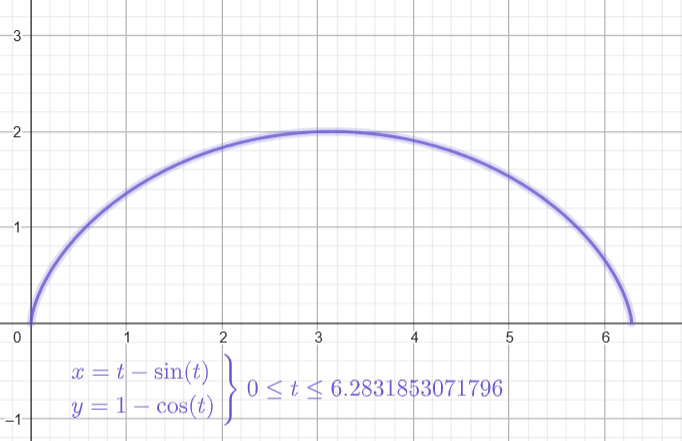
\includegraphics[width=6cm]{5J-2.1-seda.jusjajeva.INF.png}
\end{figure}



\begin{thebibliography}{999}
%\bibitem{a} Referentie
\end{thebibliography}
\end{document}